\documentclass[../main.tex]{subfiles}
\begin{document}
	
	\section{Lista 4}
		\subsection{Parte 1}
		
		\begin{exercicio}{3}
			Demonstrar a propriedade operatória do limite da soma de campos vetoriais. (Baseie-se na demonstração feita no texto para o produto escalar de campos vetoriais)
		\end{exercicio}
		\begin{solucao}
			Sejam $f,g\colon S\subset \mathbb{R}^n \rightarrow \mathbb{R}^m$ campos vetoriais e $a$ ponto de acumulação de $S$. Seja $\lim_{x \to a} f(x)=b$ e $\lim_{x \to a} g(x)=c$. Pela definição de limite de funções e pela definição da soma de funções, temos:
			\begin{align*}
				\lim_{x \to a} (f(x) \pm g(x))
					&= \lim_{x \to a} (f_1(x)\pm g_1(x),\dots, f_m(x)\pm g_m(x)) \\
					&= \lim_{x \to a} \bigg((f_1(x),\dots,f_m(x))\pm (g_1(x),\dots, g_m(x))\bigg)\\
					&= \lim_{x \to a} (f_1(x),\dots,f_m(x))\pm \lim_{x \to a} (g_1(x),\dots, g_m(x)) \\
					&= \lim_{x \to a} f(x) \pm \lim_{x\to a} g(x) \\
			\end{align*}
			$\therefore \lim_{x \to a} (f(x) \pm g(x)) = b+c$
		\end{solucao}
		
		\begin{exercicio}{4}
			Exercícios da seção 8.5 do Apostol - Calc II, pp 282-283:
			\begin{enumerate}[label=\alph*)]
				\item (1) -- resolver e ilustrar em ambiente CAS;
				\item (6) -- resolver e ilustrar em ambiente CAS;
				\item (7)
				\item (8)
			\end{enumerate}
		\end{exercicio}
		\begin{solucao}
			Antes de iniciar a solução, é interessante observar as seguintes definições:
			\begin{definicao}{Limite}
				Sejam $f(x)\colon S\subset \mathbb{R}^n\to \mathbb{R}^m$, $m\geq 1$, $a\in S$ um ponto de acumulação de $S$. Dizemos que $b$ é o limite de $f(x)$ se, quando $\|x-a\|\to 0$, temos que $\|f(x)-b\|\to 0$ e escrevemos:
				\[
				\lim_{x\to a}f(x)=b
				\]
			\end{definicao}
			\begin{definicao}{Continuidade}
				Sejam $f(x)\colon S\subset \mathbb{R}^n\to \mathbb{R}^m$, $m\geq 1$, $a\in S$ um ponto de acumulação de $S$. Dizemos que $f$ é contínua em $a$ se $f$ é definida em $a$ e
				\[
				\lim_{x\to a}f(x)=f(a)
				\]
			\end{definicao}
			\begin{enumerate}[label=\alph*)]
				\item 
				\item Se $(x,y)\neq (0,0)$, seja $f(x,y)=\tfrac{x^2-y^2}{x^2+y^2}$.
				Assim, note que ao longo da reta $y=mx$, temos
				\begin{align*}
					\lim_{(x,y)\to (0,0)} f(x,mx)
					&=\lim_{(x,y)\to (0,0)} \frac{x^2-m^2x^2}{x^2+m^2x^2}\\
					&=\lim_{(x,y)\to (0,0)}\frac{x^2(1-m^2)}{x^2(1+m^2)}\\
					&=\lim_{(x,y)\to (0,0)}\frac{1-m^2}{1+m^2}\\
					&=\frac{1-m^2}{1+m^2}
				\end{align*}
				Portanto, o limite de $f(x,y)$ quando $(x,y)\to (0,0)$ ao longo da reta $y=mx$ é $\tfrac{1-m^2}{1+m^2}$.
				
				No entanto, ao mesmo tempo, temos que, para a reta $x=0$, ou seja, para o eixo $y$,
				\begin{align*}
					\lim_{(x,y)\to (0,0)} f(0,y) 
					&=\lim_{(x,y)\to (0,0)} \frac{-y^2}{y^2}\\
					&=\lim_{(x,y)\to (0,0)} -1\\
					&=-1
				\end{align*}
				Analogamente, para a reta $y=0$, ou seja, para o eixo $x$,
				\begin{align*}
					\lim_{(x,y)\to (0,0)} f(x,0)
					&=\lim_{(x,y)\to (0,0)} \frac{x^2}{x^2}\\
					&=\lim_{(x,y)\to (0,0)}1\\
					&=1
				\end{align*}
				Dessa forma, note que o limite de $f(x,y)$ quando $(x,y)\to (0,0)$ é diferente, dependendo do caminho que tomamos. Logo, não existe um $b$ tal que, quando $\|(x,y)-(0,0)\|\to 0$, temos que $\|f(x,y)-b\|\to 0$, pois caso $b=1$, sempre existe uma sequência em $(x,y)$ tal que $f(x,y)$ converge para um número diferente $b_1=-1$, e vice-versa. Pela definição de limite, $\lim_{(x,y)\to (0,0)} f(x,y)$ não existe.
				
				Entretanto, note que, pela definição de continuidade num ponto $a=(0,0)$, $\lim_{(x,y)\to a} f(x,y)$ deve existir, e deve ser igual a $f(a)$. Como esse limite não existe, não é possível definir $f(0,0)$, de modo que $f$ seja contínua em $(0,0)$.
				Abaixo está a ilustração da função $f$ no SageMath.
				\begin{center}
					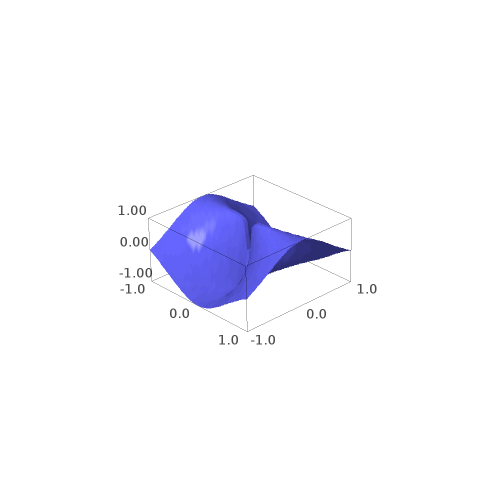
\includegraphics[width=0.25\textwidth]{imagens/lista04/picture_lista04.01_q04_item02.png}
					\captionof{figure}{$f(x,y)=\tfrac{x^2-y^2}{x^2+y^2}$}
				\end{center}
				\item
				\item Seja $f(x,y)=\tfrac{\sin(x^2+y^2)}{x^2+y^2}$ quando $(x,y)\neq (0,0)$. Queremos definir $f(0,0)$ de modo que $f$ seja contínua em $(0,0)$. Para tal, devemos verificar a existência do limite $\lim_{(x,y)\to (0,0)} f(x,y)$.
				
				Assim, seja $g(x,y)\coloneq x^2+y^2$ e $h(x)\coloneq \tfrac{\sin(x)}{x}$. Note que, pela continuidade dos polinômios e pelo limite trigonométrico fundamental,
				\begin{itemize}
					\item $\lim_{(x,y)\to (0,0)} g(x,y)=g(0,0)=0+0=0$
					\item $\lim_{x\to 0} h(x)=\lim_{z\to 0} \frac{\sin(x)}{x}=1$
				\end{itemize}
				Com isso, pela propriedade do limite de funções compostas,
				\begin{align*}
					\lim_{(x,y)\to (0,0)} f(x,y)
						&=\lim_{(x,y)\to (0,0)} \tfrac{\sin(x^2+y^2)}{x^2+y^2}\\
						&=\lim_{(x,y)\to (0,0)}h(g(x))=1
				\end{align*}
				Pela definição de continuidade, devemos definir $f(0,0)$ de modo que $\lim_{(x,y)\to (0,0)}f(x,y)=f(0,0)$. Assim, $f(0,0)\coloneq 1$.
			\end{enumerate}
		\end{solucao}
\end{document}
